\documentclass[12pt,a4paper]{article}
\usepackage[utf8]{inputenc}
\usepackage[russian]{babel}
\usepackage[OT1]{fontenc}
\usepackage{amsmath}
\usepackage{amsfonts}
\usepackage{amssymb}
\usepackage{graphicx}
\usepackage{array}
\usepackage{cancel}
\usepackage{caption}
\usepackage{wrapfig}
\usepackage{secdot}
\usepackage{indentfirst}
\usepackage[left=1.5cm,right=1.5cm,top=0.3cm,bottom=1.5cm,includefoot,footskip=1.5cm]{geometry}
\begin{document}
\textbf{
\begin{flushright}
Илья Кочергин, 626 группа
\end{flushright}}
\paragraph{\large Работа 122}
\paragraph{\Large Резонанс напряжений в последовательном контуре}
\paragraph{Цель работы:}исследование резонанса напряжений в последовательном колебательном контуре с изменяемой ёмкостью, включающее получение АЧХ и ФЧХ, а также определение основных параметров контура.
\paragraph{Оборудование:}генератор сигналов, источник напряжения, нагруженный на последовательный колебательный контур с переменной ёмкостью, двулучевой осциллограф, цифровые вольтметры.
\section{Теоретическая справка} 
\paragraph{Общие уравнения.} Рассмотрим электрическую цепь, состоящую из последовательно соединенных конденсатора с емкостью $C$ и активным сопротивлением $R_S$, катушки с индуктивностью $L$ и активным сопротивлением $R_L$ и резистора с сопротивлением $R$, которая подключена к источнику переменного тока с амплитудой напряжения $E$ и частотой $f$. Тогда общее активное сопротивление цепи $R_\Sigma$ выражается формулой
\begin{equation}
R_\Sigma = R + R_S + R_L\label{rsum},
\end{equation}
а циклическая частота $\omega$ формулой
 \begin{equation}
\omega = 2\pi f\label{omeg}.
\end{equation}
Отсюда импеданс цепи определяется выражением
\begin{equation}
Z = R_\Sigma + i\left(\omega L - \frac{1}{\omega C}\right)\label{imp},
\end{equation}
из которого можно легко найти формулу для комплексной амплитуды тока $\widehat{I}$:
\begin{equation}
\widehat{I} = \frac{\widehat{E}}{Z} = \frac{E}{R_\Sigma + i\left(\omega L - \frac{1}{\omega C}\right)}\label{Ic}.
\end{equation}
Из предыдущего выражения несложно получить формулы для комплексной амплитуды напряжения на конденсаторе $\widehat{U_C}$, а также для его амплитуды $U_C$ и сдвига фаз $\varphi_C$:
\begin{equation}
\widehat{U_C} = E\frac{R_S - \frac{i}{\omega C}}{R_\Sigma + i\left(\omega L - \frac{1}{\omega C}\right)}\label{ucc};
\end{equation}
\begin{equation}
U_C = E\sqrt{\frac{R_S^2\omega^2C^2+1}{\frac{1}{Q^2}\left(\frac{\omega}{\omega_0}\right)^2 + \left(\left(\frac{\omega}{\omega_0}\right)^2-1\right)^2}}\label{uc};
\end{equation}
\begin{equation}
\varphi_C = -\arccos\left(\frac{\frac{1}{Q}R_S\omega C - \left(\left(\frac{\omega}{\omega_0}\right)^2-1\right)^2}{\sqrt{R_S^2\omega^2+1}\sqrt{\frac{1}{Q^2}\left(\frac{\omega}{\omega_0}\right)^2 + \left(\left(\frac{\omega}{\omega_0}\right)^2-1\right)^2}}\right)\label{phic}.
\end{equation}
Здесь были использованы следующие обозначения:
\begin{equation}
\begin{cases}
\omega_0 = \frac{1}{\sqrt{LC}}\text{ - собтвенная циклическая частота контура};\\
Q = \frac{1}{R}\sqrt{\frac{L}{C}}\text{ - добротность контура}.\\ 
\end{cases}\label{redef}
\end{equation}
\paragraph{Приближение вблизи резонанса.} Как мы видим, выражения (\ref{uc}) - (\ref{phic}) являются достаточно громоздкими. Для их упрощения примем, что добротность контура велика ($Q \ge 10$) и $R_S \ll R$, и будем рассматривать поведение цепи вблизи резонанса. Тогда мы можем считать $\omega_0$ резонансной циклической частотой контура, а эти выражения примут вид:
\begin{equation}
U_C = EQ\frac{\omega}{\omega_0}\frac{1}{\sqrt{1+\left(\tau\Delta\omega\right)^2}}\label{uca};
\end{equation}
\begin{equation}
\varphi_c = -\frac{\pi}{2} + \delta - \arctg(\tau\Delta\omega)\label{pca}.
\end{equation}
Новые использованные обозначения:
\begin{equation}
\begin{cases}
\tau= \frac{2!}{\omega_0}\text{ - постоянная времени контура};\\
\delta = \arctg(RC\omega)\text{ - параметр конденсатора (см. рис. \ref{Fig1})}.\\ 
\end{cases}\label{redef2}
\end{equation}
\begin{wrapfigure}{r}{0.24\textwidth}
\centering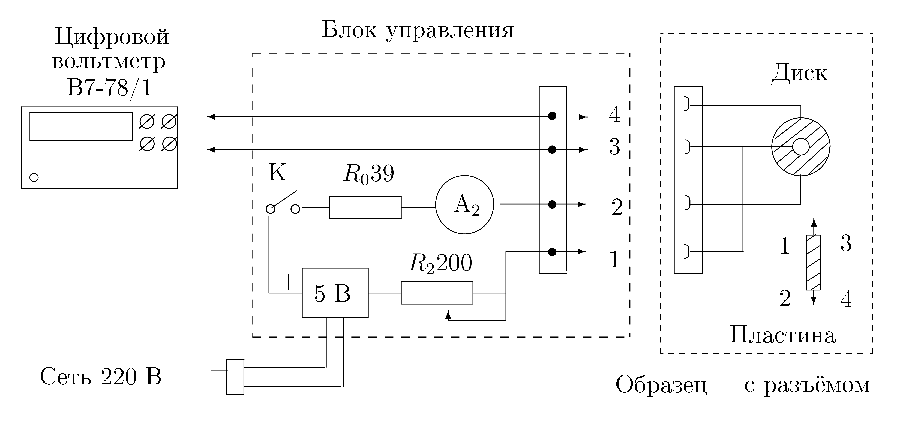
\includegraphics[width = 0.21\textwidth]{Pct1}
\captionsetup{justification = centering}
\caption{Векторная диаграмма\label{Fig1}}
\end{wrapfigure}
\end{document}